\documentclass[a4paper,11pt]{article}

\usepackage[utf8]{inputenc}

\usepackage{graphicx}
\usepackage{caption}
\usepackage{subcaption}

\usepackage{hyperref}

\usepackage{pgfplots}
\pgfplotsset{compat=1.18} 

\usepackage{minted}

\begin{document}

\title{
    \textbf{Assignment 7 Report - Queue in an Array - Java}
}
\author{Dean Tsankov}
\date{\today}

\maketitle

\section*{Introduction}

In this report I will present an alternative way to implement the Queue data structure. Instead of using a linked list as an underlying structure here I will instead rely on an array. The reason we might want to not use linked lists depends on the cost of memory allocation. With optimizing this property we introduce the fact that the implementation itself becomes a bit more complicated.

\section*{General Idea}

The main way this queue is intended to work is the following: The queue has a property which is the array holding the data and pointer values indicating the indices of the first element in the queue and the one after the last (the next possible position for enqueue-ing). When we add an element to the queue we write it at the current {\tt last} index and increment it. Conversely when removing an element we delete the data in the array at the {\tt first} index and increment it as well. 

The complications arise when we reach a {\tt last} value equal to the array length. At that point it is most probably the case that there are still a couple of empty slots before the {\tt first}. We would like to utilize this space and not mindlessly expand the array disregarding this optimisation. This will be done by, in essence, wrapping the {\tt last} index back to the beginning. The way to do this is by incrementing that index not only by 1 but then also taking its modulo with regard to the current size of the array. 

That sort of thinking allows us to fully use the current size of the array, but there will come a time when the whole array will in fact be filled. In order for us to reference this it would be useful to introduce a new property into the structure, keeping track of the actual elements in the queue. The work we do with this variable is fairly self explanatory - its increased when enqueue-ing and decreased when dequeue-ing. 

With the current wrap-around setup we will know that we are in an edge case if the first and last indices have the same value. This happens either when there are no elements in the queue, i.e we removed the last element or we are trying to add the first element, these cases should be accounted for with simple checks. The more important case is the one where we are trying to override the first value with a new element. This is when the dynamic size increase should happen. That is we transfer the data to a twice as large array. During this transfer we do not need to preserve the wrap-around order and so we can "straighten" the elements.

Essentially that is the idea of the array implementation of a queue.

\section*{The Code}

This is how the class is defined and initiated by the constructor: 

\begin{minted}[
frame=single,
framesep=2mm,
baselinestretch=1.2,
fontsize=\footnotesize,
]{java}
    (...)
    public class ArrayQueue<T> extends JQueue<T> {

    private T[] queue;
    private int first; //index of first element in queue
    private int last; //index of last element in queue
    private int size; //number of elements in queue
    public Class<T> clazz; //allows this class to use a generic array

    public ArrayQueue(Class<T> clazz) {
        this.queue = (T[]) Array.newInstance(clazz, 4);
        first = -1;
        last = -1;
        size = 0;
        this.clazz = clazz;
    }
    (...)
\end{minted}

The first and last indices are set to -1 on initiation so as to signal that the queue is empty. The class itself extends an abstract Queue class which ensures the abstraction of this implementation.

Next is the enqueue function, the most involved part of the structure:

\begin{minted}[
frame=single,
framesep=2mm,
baselinestretch=1.2,
fontsize=\footnotesize,
]{java}
    (...)
    public void enqueue(T item) {
        if (size == 0) {
            first = 0;
            last = 0;
        }
        if(last == first && size!=0){
            int n = queue.length*2;
            int tempfirst = first;
            T[] tempQueue = (T[]) Array.newInstance(clazz, n);
            for (int i = 0; i < size; i++) {
                tempQueue[i] = queue[tempfirst];
                tempfirst = (tempfirst + 1) % queue.length;
            }
            queue = tempQueue;
            first = 0;
            last = size;
        }
        queue[last] = item;
        last = (last + 1) % queue.length;
        size++;

    }
    (...)
\end{minted}

It generally follows the explanations given above. The first element case is handled by setting both indices to zero and later incrementing the {\tt last}. There is the array expansion routine and finally the actual writing to the array.

Lastly is the dequeue method:

\begin{minted}[
frame=single,
framesep=2mm,
baselinestretch=1.2,
fontsize=\footnotesize,
]{java}
    (...)
    public T dequeue() {
        if (first == -1) {
            return null;
        }
        size--;
        T temp = queue[first];
        queue[first] = null;
        first = (first + 1) % queue.length;
        if (size == 0) {
            first = -1;
            last = -1;
        }
        return temp;
    }
    (...)
\end{minted}

At first there is a check if the queue is already empty otherwise it proceeds to delete the correct data from the queue and increment the pointer. There also happens to be a peace keeping check if the removed element was the last in the queue and if so, then the indices get reset.

\section*{Benchmark}

I decided to also present a comparison between this array queue and the linked list queue I had already done for the previous assignment. This is a graphical plot of the time with respect to the amount of elements being enqueued:

\begin{figure}[H]
    \centering
    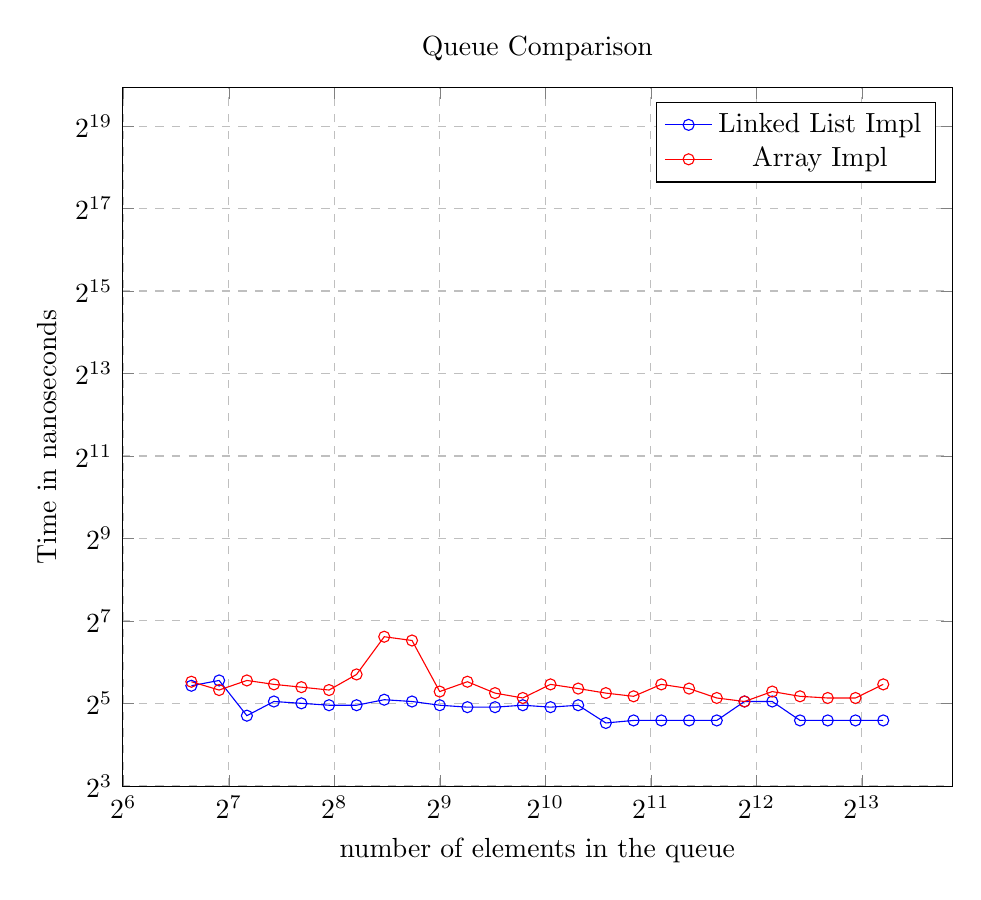
\begin{tikzpicture}
        \begin{axis}[
            title={Queue Comparison},
            width=\linewidth,
            xlabel={number of elements in the queue},
            ylabel={Time in nanoseconds},
            ymin=0, ymax=1000000,
            xmode=log,
            log basis x={2},
            ymode=log,
            log basis y={2},
            ymajorgrids=true,
            xmajorgrids=true,
            grid style=dashed,
        ]
        

        \addplot[
            color=blue,
            mark=o,
            ]
            coordinates {
            (100,43)(120,47)(144,26)(172,33)(206,32)(247,31)(296,31)(355,34)(426,33)(511,31)(613,30)(735,30)(882,31)(1058,30)(1269,31)(1522,23)(1826,24)(2191,24)(2629,24)(3154,24)(3784,33)(4540,33)(5448,24)(6537,24)(7844,24)(9412,24)
            };
            \addlegendentry{Linked List Impl}

        \addplot[
            color=red,
            mark=o,
            ]
            coordinates {
            (100,46)(120,40)(144,47)(172,44)(206,42)(247,40)(296,52)(355,98)(426,92)(511,39)(613,46)(735,38)(882,35)(1058,44)(1269,41)(1522,38)(1826,36)(2191,44)(2629,41)(3154,35)(3784,33)(4540,39)(5448,36)(6537,35)(7844,35)(9412,44)
            };
            \addlegendentry{Array Impl}
            
            
        \end{axis}
        \end{tikzpicture}
    \caption{Queue Comparison}
    \label{fig:plot1}
\end{figure}

\section*{Conclusion}

It is generally apparent that the array implementation requires more time, since it is expanding its size quite a few times while the linked list has a constant cost for adding elements. Even still the array implementation also has a constant time complexity since its expand operations get amortised. The difference between the two alternatives will become apparent when we consider the memory accesses and the amount of cash misses the linked list yields each time it operates on the queue.

\end{document}